% Chapter 4

\chapter{Hiện thực hệ thống} % Main chapter title

\label{Chapter4}

\section{Thiết kế cơ sở dữ liệu}
\subsection{Mô hình quan hệ thực thể}
Hệ thống gồm các thực thể chính:
\begin{itemize}
    \item Node
    \item Segment
    \item Cell
    \item Street
    \item Traffic Status
\end{itemize}
\begin{figure}[H]
\centering
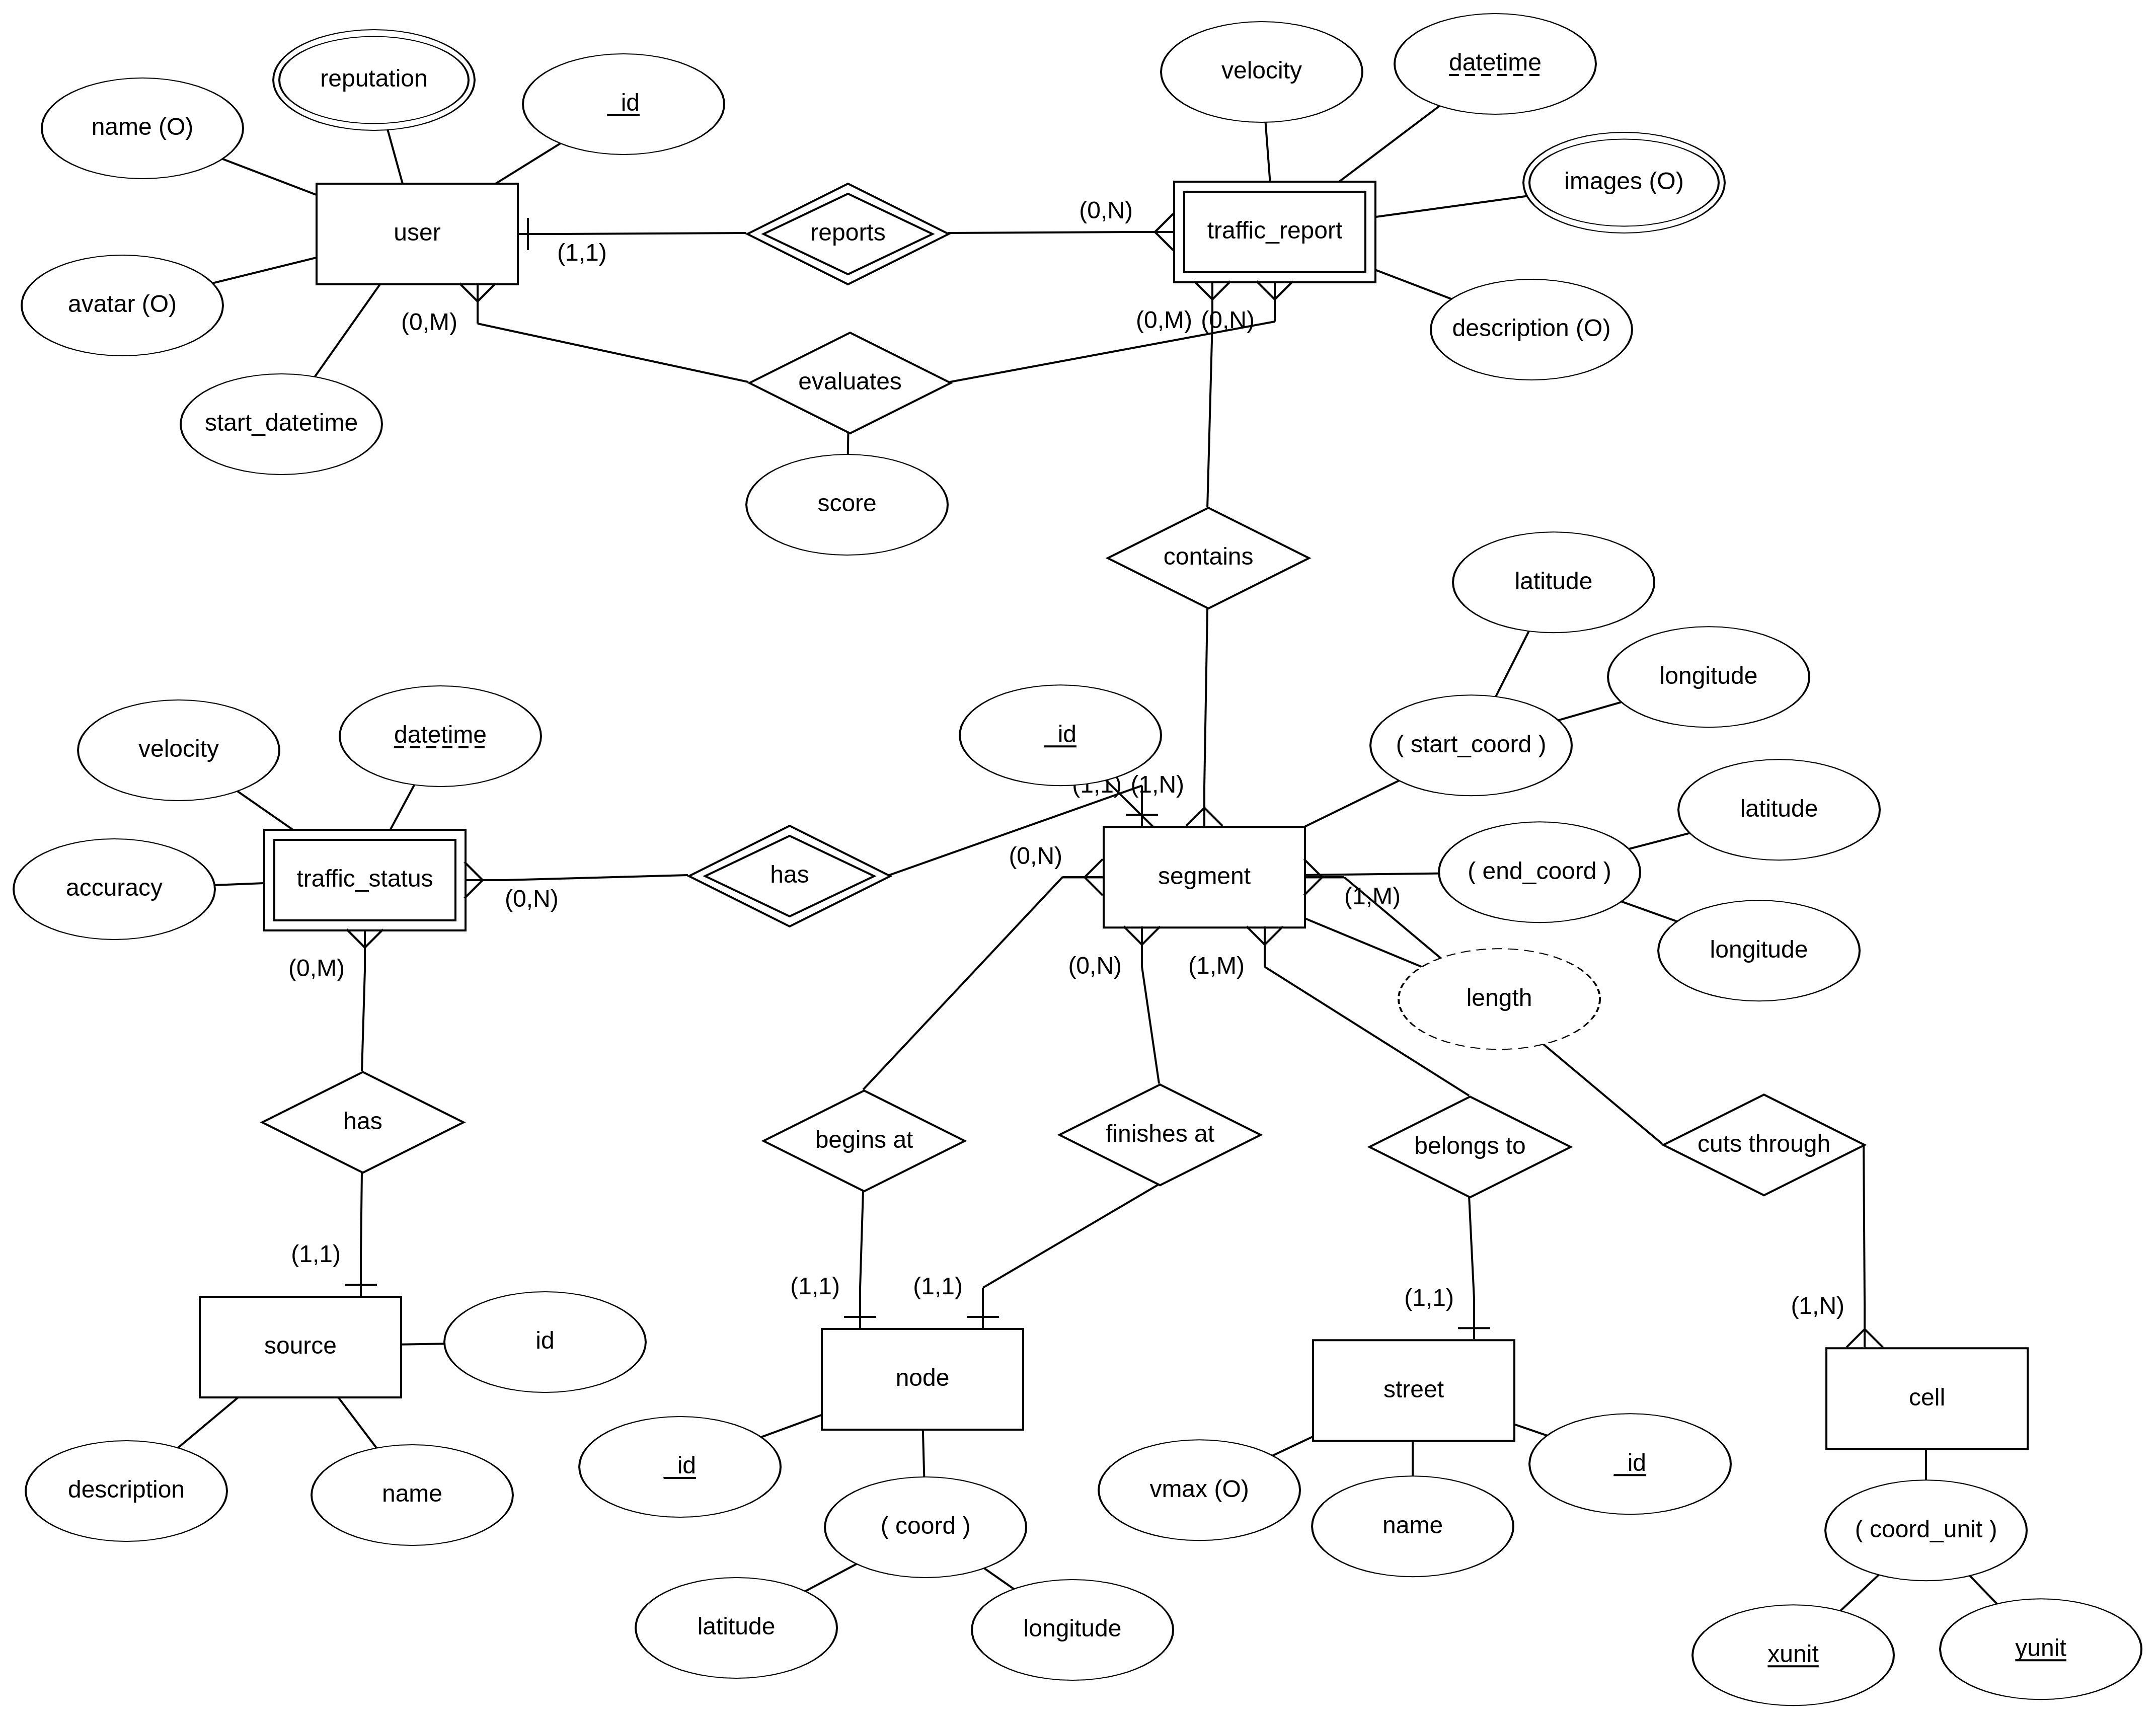
\includegraphics[width=1.0\textwidth]{Traffic_Report/images/erd.png}
\caption{Mô hình quan hệ thực thể}\label{}
\end{figure}

\subsection{Phân tích thực thể}
\textbf{node:} là một \textit{điểm} trên bản đồ được quy định sẵn bởi OpenStreetMap, gồm:
\begin{itemize}
    \item \lstinline{id:int}: định danh node.
    \item \lstinline{coord (latitude:float, longtitude:float)}: toạ độ node, gồm vĩ độ và kinh độ.\\
\end{itemize}

\textbf{segment:} là đơn vị nhỏ nhất để đánh giá tình trạng giao thông. Mỗi segment là một đoạn nối 2 node đầu - cuối, gồm:
\begin{itemize}
    \item \lstinline{id:int}: định danh segment.
    \item \lstinline{start_coord (latitude:float, longtitude:float)}: toạ độ gồm vĩ độ, kinh độ của node đầu.
    \item \lstinline{end_coord (latitude:float, longtitude:float)}: toạ độ gồm vĩ độ, kinh độ của node cuối.
    \item \lstinline{length:int}: chiều dài segment tính theo mét, có thể tính dựa vào toạ độ 2 node đầu - cuối\\
\end{itemize}

\textbf{cell:} được đưa ra để thuận tiện trong việc xác định các node, segment. Khi có toạ độ một đoạn đường có thể dựa vào cell để ánh xạ ra các segment thuộc đoạn đường đó. Mỗi cell là ô vuông có cạnh 100m, gồm:
\begin{itemize}
    \item \lstinline{coord_unit (xunit:int, yunit:int)}: chỉ số toạ độ của cell theo trục x và y. Gốc toạ độ O là một điểm được quy định trước.\\
\end{itemize}
Mỗi cell có thể chứa nhiều segment và tương tự, mỗi segment cũng có thể nàm trong nhiều cell, tuỳ thuộc vào độ dài và vị trí của segment.

\textbf{street:} mỗi street (con đường) chứa nhiều segment liên tiếp nhau, gồm:
\begin{itemize}
    \item \lstinline{id:int}: định danh street.
    \item \lstinline{name:string}: tên street.
    \item \lstinline{vmax(O):int}: tốc độ tối đa cho phép trên street đó tính theo km/h, có thể null.\\
\end{itemize}

\textbf{traffic\_status:} là tình trạng giao thông tại một segment vào một thời điểm. Vì vậy traffic\_status là một thực thể yếu của segment, gồm:
\begin{itemize}
    \item \lstinline{datetime:timestamp}: thời gian (ngày giờ) của tình trạng giao thông đó.
    \item \lstinline{velocity:int}: tốc độ lưu thông.
    \item \lstinline{accuracy:float}: sai số tốc độ.\\
\end{itemize}

Ngoài ra còn có \textbf{time\_frame:} là một bảng tham chiếu khung giờ được chia sẵn, có thể thay đổi mỗi frame là 10 hay 15 phút...\\

Phạm vi của đề tài này là tập trung vào phân tích và dự đoán giao thông, nên phần chi tiết liên quan đến \lstinline{source} và \lstinline{traffic_report} (thuộc về crowdsourcing) nhóm không đề cập đến.

\section{Ước lượng vận tốc ở các segment không thu thập được dữ liệu}

\section{Xây dựng ứng dụng web}
\subsection{Tổng quan}
Ở giai đoạn phát triển đề cương luận văn, nhóm nghiên cứu mới chỉ bước đầu xây dựng trang web hiển thị tình trạng giao thông từ dữ liệu lấy được qua các API của hệ thống Smart BK Traffic.
\subsection{Ứng dụng web (Front-end)}
Về phía Front-end, nhóm sử dụng OpenStreetMap API để tạo map cơ bản, đồng thời sử dụng thư viện Leaflet để hỗ trợ việc thêm các đường thẳng, điểm đánh dấu lên map để biểu diễn tình trạng giao thông.

\begin{figure}[!ht]
	\begin{center}
		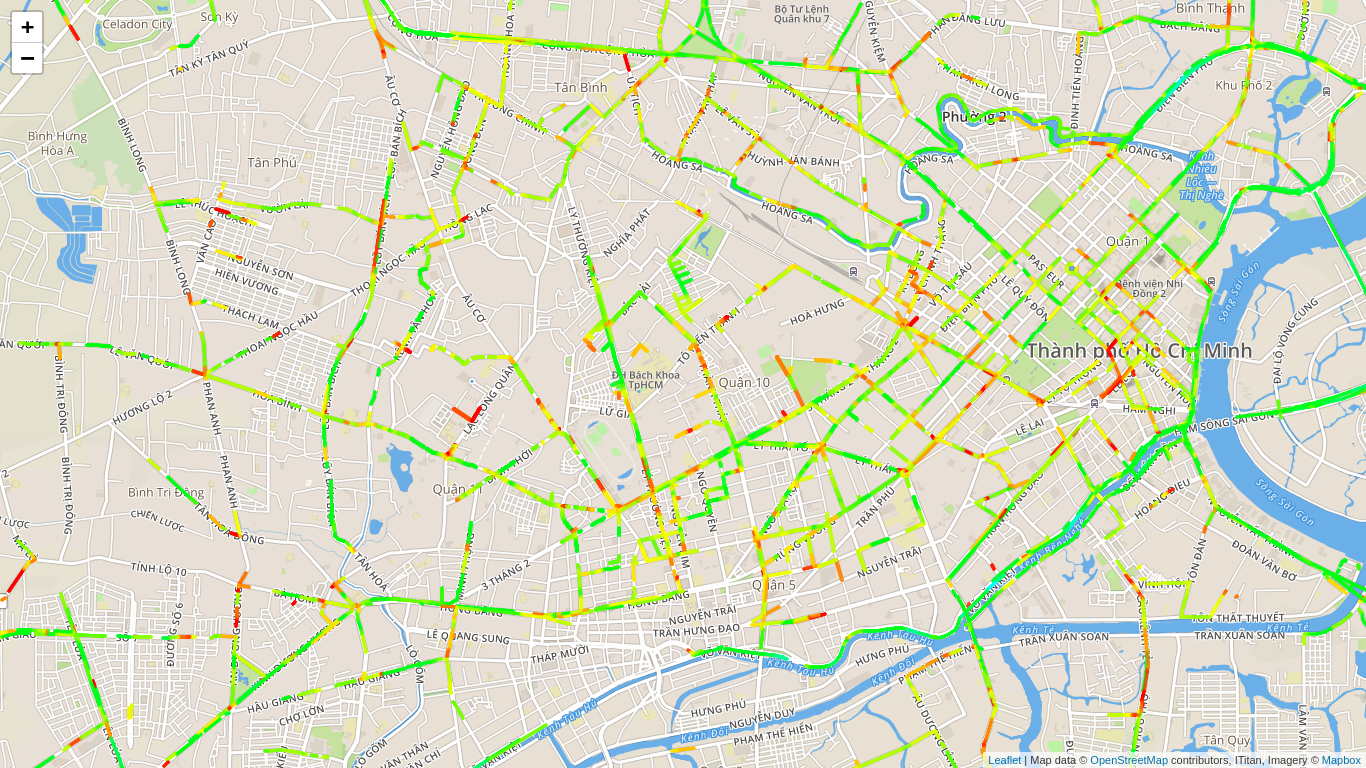
\includegraphics[width=1.0\textwidth]{Traffic_Report/images/map.png}
	\end{center}
	\caption{Web application thể hiện tình trạng giao thông}
\end{figure}

Khi người dùng truy cập vào địa chỉ web, browser sẽ thực hiện xác định tọa độ 4 góc của map đang hiển thị, gửi các tọa độ đó về cho server để thực hiện lấy dữ liệu và tạo các đoạn màu trên map dựa trên dữ liệu lấy được để biểu diễn tình trạng giao thông. Cụ thể, tùy theo trường vận tốc mà chúng ta có dãy màu để biễu diễn như sau:

\begin{figure}[!ht]
	\begin{center}
		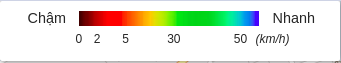
\includegraphics[width=0.5\textwidth]{Traffic_Report/images/color.png}
	\end{center}
	\caption{Dãy màu thể hiện tốc độ luồng giao thông}
\end{figure}

Cơ chế biểu diễn tốc độ luồng giao thông bằng dãy màu khá đơn giản, cụ thể như sau:
\begin{itemize}
    \item Với v < 0: hệ thống trả về màu #FF0000 (màu đỏ).
    \item Với 0 < v < 10: hệ thống sẽ trả về dãy màu #FFxx00 (màu đỏ đến màu vàng), trong đó xx phụ thuộc vào vận tốc mà sẽ có giá trị chạy từ 00 đến FF.
    \item Với 10 < v < 40: hệ thống sẽ trả về dãy màu #xxFF00 (màu vàng đến màu xanh lá cây), trong đó xx phụ thuộc vào vận tốc mà sẽ có giá trị chạy từ FF đến 00.
    \item Với 40 < v < 60: hệ thống sẽ trả về dãy màu #00FFxx (màu xanh lá cây đến màu xanh dương nhạt), trong đó xx phụ thuộc vào vận tốc mà sẽ có giá trị chạy từ 00 đến FF.
    \item Với x $\geq$ 60: hệ thống sẽ trả về màu xanh dương đậm.
\end{itemize}
\subsection{Server (Back-end)}
Về phía server, nhóm cũng chỉ viết một số API để hỗ trợ việc lấy dữ liệu giao thông, cũng như tạo một chương trình nhỏ chạy song song để thực hiện get dữ liệu toàn thành phố lưu trữ vào database mongodb như đã trình bày ở phần 4.1.

Dưới đây là danh sách một số API tạm thời mà nhóm đã viết:
\begin{itemize}
    \item \textbf{API @GET /api/all}
    \begin{itemize}
        \item Tên: getAll
        \item Miêu tả: Lấy tất cả dữ liệu traffic status đã lưu vào mongodb
        \item Input: Không
        \item Output: JSON Object gồm danh sách các trạng thái giao thông đã lưu trong dữ liệu mongodb.
    \end{itemize}
    
    \item \textbf{API @GET /api/get}
    \begin{itemize}
        \item Tên: getBKTraffic
        \item Miêu tả: Lấy dữ liệu giao thông gián tiếp thông qua API của Smart BK Traffic. 
        \item Input:
        \begin{itemize}
            \item @latTL: vĩ độ điểm góc trên cùng bên trái
            \item @lonTL: kinh độ điểm góc trên cùng bên trái
            \item @latTR: vĩ độ điểm góc trên cùng bên phải 
            \item @lonTR: kinh độ điểm góc trên cùng bên phải
            \item @latBL: vĩ độ điểm góc dưới cùng bên trái
            \item @lonBL: kinh độ điểm góc dưới cùng bên trái
            \item @latBR: vĩ độ điểm góc dưới cùng bên phải
            \item @lonBR: kinh độ điểm góc dưới cùng bên phải 
            \item @zoom: độ zoom của map
        \end{itemize}
        \item Output: JSON Object gồm danh sách các trạng thái giao thông được lấy từ API hệ thống Smart BK Traffic.
    \end{itemize}
    
    \item \textbf{API @GET /api/update}
    \begin{itemize}
        \item Tên: updateBKTraffic
        \item Miêu tả: Lấy dữ liệu giao thông bị thiếu khi sử dụng API /api/get
        \item Input:
        \begin{itemize}
            \item @key: tham số dùng để lấy dữ liệu bị thiếu của hệ thống Smart BK Traffic.
        \end{itemize}
        \item Output: JSON Object gồm danh sách các trạng thái giao thông được lấy từ API hệ thống Smart BK Traffic.
    \end{itemize}
\end{itemize}